\documentclass[aspectratio=1610, xcolor=dvipsnames]{packages/beamer}
%\input{smile_styles}
\usepackage[nolist,nohyperlinks]{acronym}


\usetheme{Madrid}
\useinnertheme{circles}
\useoutertheme{infolines}
\usefonttheme{serif}
\usepackage{etoolbox}
\definecolor{UBMaroon}{rgb}{0.3, 0.0, 0.0} % UBC Blue (primary)
\definecolor{UBBlackPurple}{rgb}{0.1, 0.07, 0.12} % UBC Blue (primary)
\usecolortheme[named=UBBlackPurple]{structure}

% \usepackage[cache=false]{minted}
\usepackage{amsthm}
\usepackage{amsmath}
\usepackage{amssymb,mathtools}
\usepackage[longend]{algorithm2e}
\usepackage{textgreek}
\usepackage{tcolorbox}
\usepackage{listings}
\usepackage{textcomp}
\usepackage[style=authortitle,backend=biber]{biblatex}
\usepackage{caption}
\usepackage{subcaption}
\usepackage{color}
\usepackage{graphicx}
\newcommand{\displayTOC}{\begin{frame}\frametitle{Agenda} \tableofcontents[currentsection, subsectionstyle=show/show/hide]\end{frame}}
\newcommand{\argmax}{\operatornamewithlimits{argmax}}
\newcommand{\jointS}{\bar{\mathbf{S}}}
\newcommand{\jointA}{\bar{\mathbf{A}}}
\newcommand{\joints}{\bar{s}}
\newcommand{\jointa}{\bar{a}}
\newcommand{\add}{\textcolor{red}}

% \newcommand{\joint}[1]{\bar{#1}}
\newcommand{\joint}[1]{#1}



\addbibresource{packages/references.bib}
\hypersetup{
        unicode=true,
        linkcolor=blue,
        anchorcolor=blue,
        citecolor=green,
        filecolor=black,
        urlcolor=blue
    }


%#########################################################
%#########################################################
%#########################################################
\title{Update <date start> - <date end>}\author{Mason Smith}\date\today
\begin{document}\begin{frame}[plain]\titlepage\end{frame}


\begin{acronym}
    \acro{RL}{reinforcement learning}
    \acro{QRE}{Quantal Response Equilibrium}
     \acro{ToM}{Theory of Mind}
     \acro{AUIC}{area under the indifference curve}
     \acro{CPT}{cumulative prospect theory}
\end{acronym}




%%%%%%%%%%%%%%%%%%%%%%%%%%%%%%%%%%%%%%%%%%%%%%%%%%%%%%%%%%%
%%%%%%%%%%%%%%%%%%%%%%%%%%%%%%%%%%%%%%%%%%%%%%%%%%%%%%%%%%%
%%%%%%%%%%%%%%%%%%%%%%%%%%%%%%%%%%%%%%%%%%%%%%%%%%%%%%%%%%%
\section{Introduction} \displayTOC

\begin{frame}{Introduction}
    Current Work: \begin{itemize}
        \item Improving game design to allow for consistent training
        \item Training stable CPT value functions that represent biased policies
        \item Redesigning world and retraining to ensure non-trivial differences
        \begin{itemize}
            \item Do not complete opposite or identical realization of strategy
            \item Want to achieve the objective (catch the target) with semi-similar success rate in different ways (trajectories)
        \end{itemize}
        \item Testing effects of assuming different biases for H in simulation
    \end{itemize}
    Challenges: \begin{itemize}
        \item Was struggling with getting stuck in local optima due to sparse gains (catch at end of game) and frequent penalties (throughout the game)

        \item There is a sensitive and fine balance for the following hyper-parameters that induce interesting policies to contrast:
        \begin{itemize}
            \item Admissible bounds for risk-sensitivity
            \item World design and initial conditions
            \item Learning hyper-parameters
        \end{itemize}
    \end{itemize}

\end{frame}

%#########################################################
%#########################################################
%#########################################################
\section{Game Design Update} \displayTOC

\subsection{Issues with Current Game}
\begin{frame}{Issues with Current Game}
    \begin{itemize}
        \item Algorithm gets stuck in local optima due to sparse gains (catch at end of game) and frequent penalties (throughout the game)
        \item Strong encouragement to wait out the rest of the game once a penalty is received (do not chase target anymore)
        \item Different worlds induced differences in bias policies that were either
        \begin{itemize}
            \item too strong
            \begin{itemize}
                \item risk-averse had 0\% catch rate while risk-seeking had 100\% catch rate
                \item impossible to evaluate coordination since strategies were incompatible $\rightarrow 0$\% catch
                \item produced trivial result since both of the incorrect assumptions had same outcome
            \end{itemize}
            \item too weak
            \begin{itemize}
                \item both policies either had near 100\% or both had 0\% performance
                \item solution is so obvious that CPT does not change it
                \item again produced trivial result due similarity between strategies
            \end{itemize}
        \end{itemize}
    \end{itemize}
\end{frame}


\subsection{Update Goals}
\begin{frame}{Update Goals}
\begin{itemize}
        \item Produce two policies (averse and seeking) that
        \begin{itemize}
            \item produce compatible strategies that achieve the objective $p(success) - \epsilon > 0$ when paired
            \item produce sufficiently unique joint-behavior when mis-matching policies compared to matching policies
            \item produce sufficiently similar performance between matched-averse and matched-seeking policies s.t. comparison between is valid
        \end{itemize}
        \item Modify
        \begin{itemize}
             \item world configurations (initial positions and penalty positions)
             \item global game rules and game hyper-parameters
        \end{itemize}
    \end{itemize}
\end{frame}

\subsection{List of Updates}
\begin{frame}{List of Updates}
    \begin{itemize}
        \item Redesigned world initial states and penalty locations
        \begin{itemize}
            \item remove low-effect and difficult to train worlds
        \end{itemize}
        \item Reward for catching target $r(catch)= 20 \rightarrow 25$
        \begin{itemize}
            \item increasing window to receive positive reward $\sum r_{t} >0$ after penalties and $-1$ turn reward are added
        \end{itemize}
        \item Reward is now delivered as a single cumulative reward $r_\zeta$ at the end of the game
        \begin{itemize}
            \item previously provided reward at every time-step $r_{t}$
            \item helps avoid getting stuck local optima since intermediate rewards were only penalties
            \item evaluates reward on a trajectory-scope $r_\zeta(\mathbf{s}_T,\mathbf{a}_T)$
            \item instead of action-scope $r_{t}(s_t,a_t)$ where $r_\zeta = \sum_{t\in T} \; r_t$
            \item apply eligibility traces ($TD(\lambda)$) to account for increased sparsity
        \end{itemize}
        \item Reward is now non-negative
        \begin{itemize}
            \item the cumulative reward at the end of the game is $r_\zeta = max(r_\zeta,0)$
            \item new objective is to maximize your reward \textbf{upon catching the target}
            \item doing really bad and not catching the stag are now equivalent
            \item eliminates trivial policy of avoiding rewards by never moving (especially relevant in averse-conditions)
        \end{itemize}
    \end{itemize}
\end{frame}

\subsection{Updated Worlds}
\begin{frame}{Updated Worlds}
    \begin{figure}
        \centering
        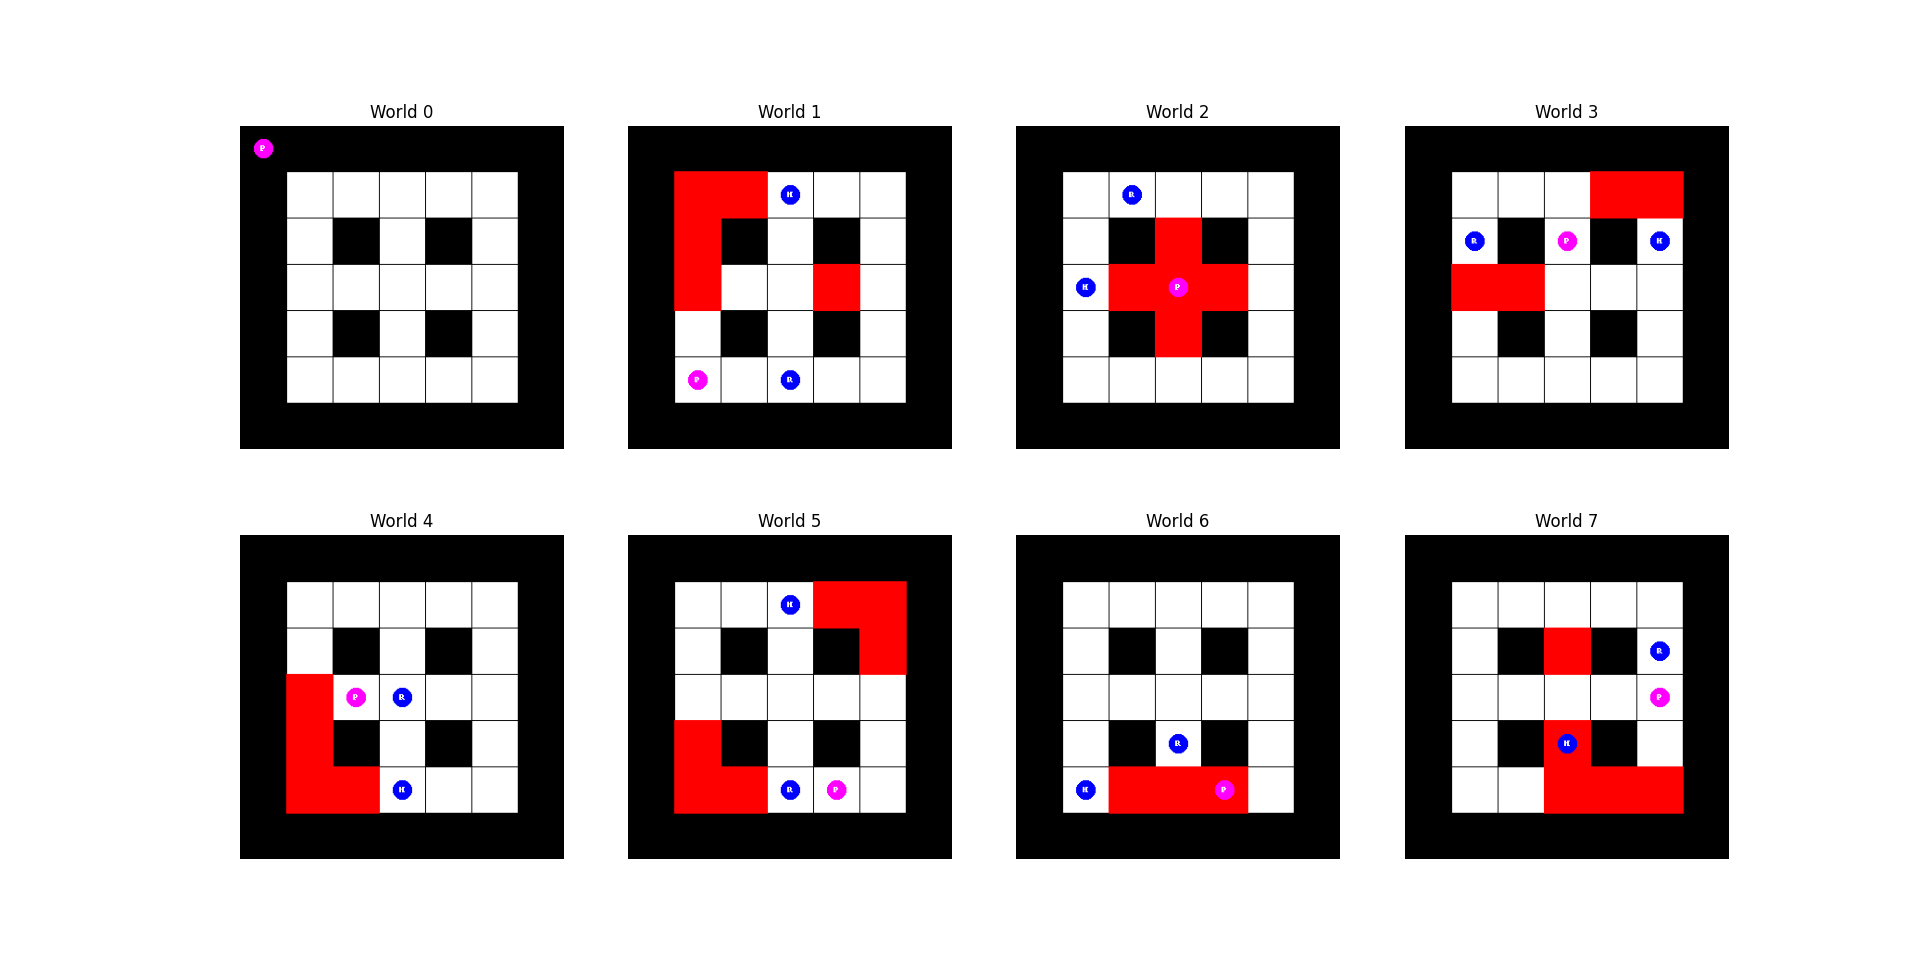
\includegraphics[width=0.95\textwidth]{../results/Fig_Worlds}
        \caption{Updated World Designs}
        \label{fig:Worlds}
    \end{figure}

\end{frame}
%#########################################################
%#########################################################
%#########################################################
\section{Training Policies} \displayTOC



\subsection{Training Setup} \begin{frame}{Training Setup}
    \begin{itemize}
        \item Implemented a independent joint-Q learning algorithm with directed exploration and \ac{ToM}
        \item \Ac{QRE} used as the equilibrium condition to solve games at every stage (\ac{ToM})
        \item Trained 3x policies $\pi$ trained during self-play:
        \begin{itemize}
            \item baseline/optimal ($\pi_{0}$)
            \item risk-averse ($\pi_{A}$)
            \item risk-seeking ($\pi_{S}$)
        \end{itemize}
        \item Baseline policy $\pi_{0}$ was used as prior for biased policies $\pi_{A}$ and $\pi_{S}$ trained with \ac{CPT} agents
        \item Sophistication (level of recursion) was set to 3 in the \ac{QRE}
    \end{itemize}
\end{frame}

\subsection{Algorithm}

\begin{frame}{Notation}
\begin{itemize}
    \item ego agent denoted by subscript $(\cdot)_k$ where $(\cdot)_{-k}$ represents the partner
    \item joint state $\joint{s} \in \joint{S}$ where $ \joint{S} = S_{k} \times S_{-k}$ given $\times$ denotes the Cartesian product
    \item joint action $\joint{a} \in \joint{A}$ where $ \joint{A} = A_{k} \times A_{-k}$ and $\joint{a}$ may be written as $\{a_k,a_{-k}\}$ for clarity
    \item ego stage reward $r_t$
    \item a policy $\pi_k$
    \begin{itemize}
        \item always denotes choosing ego action $a_k$ in $\joint{s}$
        \item samples $a_k$ from \textit{joint state-joint action} values $Q_k(\joint{s},\joint{a})$ given an est. $-k$ policy $\hat{\pi}_{-k}$
        \item $Q_k(\joint{s},\joint{a})$ is reduced to \textit{joint state-ego action} values $Q_k(\joint{s},a_k)$ by conditioning on $\hat{\pi}_{-k}$
        \begin{itemize}
            \item[]  s.t. $Q_k(\joint{s},a_k) = \mathbb{E}\big[Q_k(\joint{s},\joint{a} | \joint{a} = \{a_k,a_{-k}=\hat{\pi}_{-k}(\joint{s})\})\big]\; \forall a_k \in A_k$
        \end{itemize}
        \item $a_k$ is then drawn from $Q_k(\joint{s},a_k)$ according to a nominal Boltzmann distribution.
        \item for brevity this reduction will be implied and we will write $Q_k(\joint{s},\{a_k,\hat{\pi}_{-k}(\joint{s})\})$ to denote the full expression
        $\mathbb{E}\big[Q_k(\joint{s},\joint{a} | \joint{a} = \{a_k,a_{-k}=\hat{\pi}_{-k}(\joint{s})\})\big]\; \forall a_k \in A_k$
    \end{itemize}
   \item let $e_k(\joint{s},\joint{a})$ denote an eligibility trace keeping track of state visitations within an episode that decays by $\lambda$ each step

    % \item is the vectorized index of agent actions $\joint{a}=\joint{A}(\{a_k,a_{-k}\})$
\end{itemize}

\end{frame}

\begin{frame}{Algorithm}
    {\small
        \begin{tcolorbox}[fonttitle=\bfseries, title=Joint-$TD(\lambda)$ ]
        \begin{algorithm}[H]
        Initialize $Q_k(\joint{s},\joint{a})$ arbitrarily for all $\joint{s},\joint{a}$ \\
        \ForEach{episode}{
            Initialize $\joint{s}$ and $e_k(\joint{s},\joint{a}) = \mathbf{0}$  \\
            \ForEach{step of episode}{
                $a_k \leftarrow$ ego action given by $\pi_{k}(\joint{s} | \hat{\pi}_{-k}(\joint{s}))$ \\
                Take action $a_k$, observe joint action $\joint{a}$, ego reward $r_{k}$, and next state $\joint{s}'$ \\
                % $\delta \leftarrow r+\gamma Q_k(\joint{s}',\joint{a}') - Q_k(\joint{s},\joint{a}) $ \\
                % $\delta \leftarrow r+\gamma\max_{a'_k} \mathbb{E}\{Q_k(\joint{s}',\{a'_k,a'_{-k}\} | a'_{-k} = \hat{\pi}_{-k}(\joint{s}'))\}  - Q_k(\joint{s},\joint{a}) $ \\
                % $\delta \leftarrow r_k+\gamma\max_{a'_k} \mathbb{E}\big[Q_k(\joint{s}',\joint{a}' | \joint{a}' = \{a'_k,\hat{\pi}_{-k}(\joint{s}')\})\big]  - Q_k(\joint{s},\joint{a}) $ \\
                $\delta \leftarrow r_k+\gamma\max_{a'_k} Q_k(\joint{s}',\{a'_k,\hat{\pi}_{-k}(\joint{s}')\})  - Q_k(\joint{s},\joint{a}) $ \\
                $e_k(\joint{s},\joint{a}) \leftarrow e_k(\joint{s},\joint{a}) +1$ \\
                \ForEach{\joint{s} \times \joint{a}}{
                    $ Q_k(\joint{s},\joint{a}) \leftarrow  Q_k(\joint{s},\joint{a}) + \alpha \delta  e_k(\joint{s},\joint{a})$\\
                    $e_k(\joint{s},\joint{a}) \leftarrow \gamma \lambda e_k(\joint{s},\joint{a}) $ \\
                }
                $\joint{s},\joint{a} \leftarrow \joint{s}',\joint{a}'$ \\
                Until $\joint{s}$ is terminal \;
            }
        }
        \label{alg:algorithm}
        \end{algorithm}
        \end{tcolorbox}
    \par}
\end{frame}






\begin{frame}{Area Under the Indifference Curve (AUIC)}

        \begin{itemize}
            \item \ac{AUIC} is an expression of preference for accepting or rejecting a gamble over actions with certain outcomes in terms of probabilities $p(accept)$
            \item \ac{AUIC} is evaluated over the space of feasible rewards $\mathbf{R}$ found in the game
            \item We define binomial-choices ($a_1,a_2$) with outcomes sampling from $\mathbf{R}$ s.t. $\mathbf{R}_{1},\mathbf{R}_{2} = \mathbf{R}$
            \item The outcomes of each choice are then:
            \begin{itemize}
                \item $a_{1}$ containing one certain outcome
                \begin{itemize}
                    \item  with possible rewards $\mathbf{R}_{1} = \{r_1 -0.5*r_{\rho} \;\forall\; r_1 \in \mathbf{R}_{1}\}$
                \end{itemize}
                \item $a_{2}$ containing two uncertain outcomes (with and without a penalty $r_\rho$)
                \begin{itemize}
                    \item with possible rewards $\mathbf{R}_{2} = \{[r_2,(r_2 -r_\rho)] \;\forall\; r_2 \in\mathbf{R}_2\}$
                    \item with probabilities $p = [(1-p_{\rho}),p_{\rho}]$ for each outcome occurring
                \end{itemize}
            \end{itemize}
            \item \textit{Indifference Curve}:
            \begin{itemize}
                \item a continuous curve through the 2D reward space ($\mathbf{R}_{1} \times \mathbf{R}_{2}$)
                \item occurs when no preference is expressed s.t. $p(accept) = 1-p(accept)$
            \end{itemize}

        \end{itemize}
\end{frame}


\begin{frame}{Area Under the Indifference Curve (AUIC)}
        \begin{itemize}
        \item $p(accept)=p(a_2)$ then implies risk-sensitivity where
            \begin{itemize}
                 \item An optimal agent expresses no preference (indifferent) given $r_1=r_2 \;\forall\; r_1,r_2 \in \mathbf{R}$
                 \item Preferences become more complex as we apply CPT transformation $\mathbb{C}[\cdot]$
            \end{itemize}


            \item \ac{AUIC} will be calculated as follows:
            \begin{itemize}
                 \item Expresses the cumulative (mean) probability of $p(accept)$ across a symmetrical space of rewards transformed by CPT
                \item Centered around $0$ for legibility s.t. AUIC$\in (-0.5,0.5)$
                \item \ac{AUIC} $=\frac{1}{|\mathbf{R}_1 \times \mathbf{R}_2|} \sum_{r_1,r_2\in \mathbf{R}_{1},\mathbf{R}_{2}}  p(accept | \mathbb{C}[r_1,r_2]) - 0.5$
            \end{itemize}
            % expressed as the centered, mean transformation of CPT[$\mathcal{P}_{CPT}$] on AUIC$ = p(accept)-0.5$ s.t. AUIC$\in (-0.5,0.5)$
            \item The value for \ac{AUIC} can then be interpreted as follows:
            \begin{itemize}
                \item $\text{\ac{AUIC}}+p_{\epsilon} < 0$: the agent cumulatively prefers rejecting the gamble and is risk-averse
                \item $\text{\ac{AUIC}}-p_{\epsilon} > 0$: the agent cumulatively prefers accepting the gamble and is risk-seeking
                \item $|\text{\ac{AUIC}}| < p_{\epsilon}$: the agent agent has week cumulative preferences and is risk-insensitive
                \item $\text{\ac{AUIC}} = 0$: the agent has no cumulative preferences and is optimal
                \item where $p_{\epsilon}=0.1$ is a threshold defining what we consider risk-sensitive
            \end{itemize}


        \end{itemize}

\end{frame}

\begin{frame}{Area Under the Indifference Curve (AUIC)}
     \begin{figure}
        \centering
        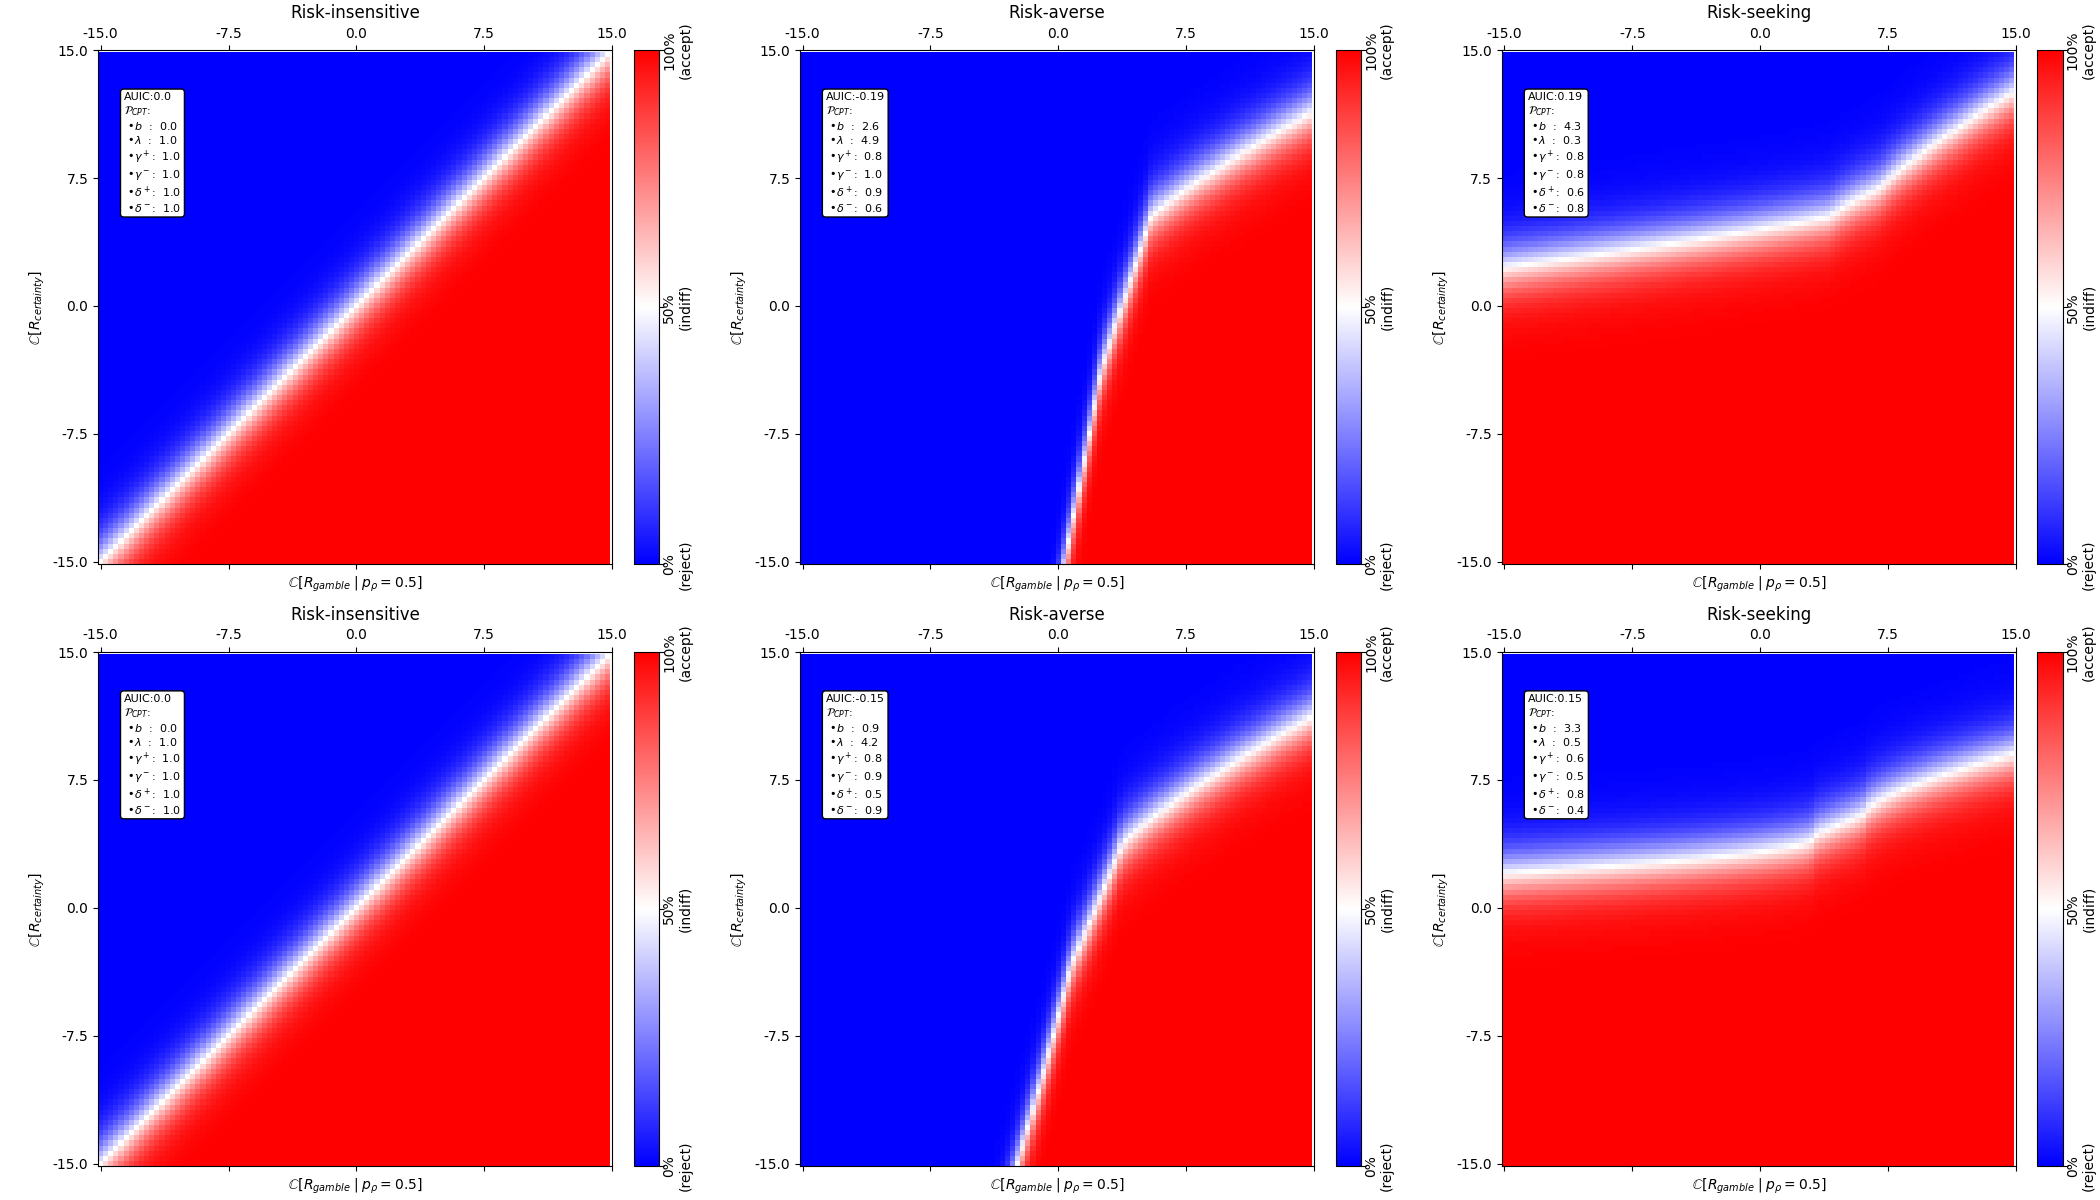
\includegraphics[width=0.95\textwidth]{../results/Fig_AUIC}
        \caption{AUIC Samples}
        \label{fig:AUIC}
    \end{figure}

\end{frame}


\subsection{Creating Biased Policies}\begin{frame}{Creating Biased Policies}
    \begin{itemize}
        \item \Ac{CPT} parameters $\mathcal{P}_{CPT}$ were stochastically perturbed while training biased policies
        \begin{itemize}
            \item $\mathcal{P}_{CPT}$ were sampled in batches every 200 episodes
            \item $\mathcal{P}_{CPT}$ were sampled from feasible bounds based on behavioral research \add{[CITE]}
            \item $\mathcal{P}_{CPT}$ were attributed to averse or seeking behavior based on the \ac{AUIC}
        \end{itemize}
        \item $\mathcal{P}_{CPT}$ is continuously sampled until intended risk-sensitivity (\text{\ac{AUIC}}) is met
    \end{itemize}
\end{frame}



\subsection{Results}
\begin{frame}{Convergence Expectations}
    \begin{itemize}
        \item "Optimal strategy" is arbitrary between different bias conditions
        \item Different bias conditions induce different environment and therefore different policy
        \item Convergence conditions and final policy performance is not shared between bias conditions
        \item Seeking and baseline strategies may be similar due to world conditions
        \item It is somewhat hard to tell if a policy has converged for the averse condition $\pi_A$
        \begin{itemize}
            \item Obvious convergence is not present.
            \item averse induces higher penalties and less value in entering penalty states to chase target
            \item Convergence often not evident from rewards, episode length, or probability of catching the target + MARL environments can be non-stationary
            \item instead, relies on several iterations with varying learning parameters converging to similar results
            \item had to update worlds\footnote{This took considerable time to find this balance s.t. differences between conditions were non-trivial} to balance between the risk of entering penalty states and the gain from doing so conditioned on uncertainty about partner motion to get a non-trivial policy (no movement = optimal)
        \end{itemize}

    \end{itemize}
\end{frame}


% ########## BEGIN RESULTS FIGURES #####################
\newcommand{\Wfig}{0.48}

\begin{frame}{Training Results (World 1)}
     \begin{figure}
     \centering
        %  \begin{subfigure}[b]{\Wfig\textwidth}  \centering
        %      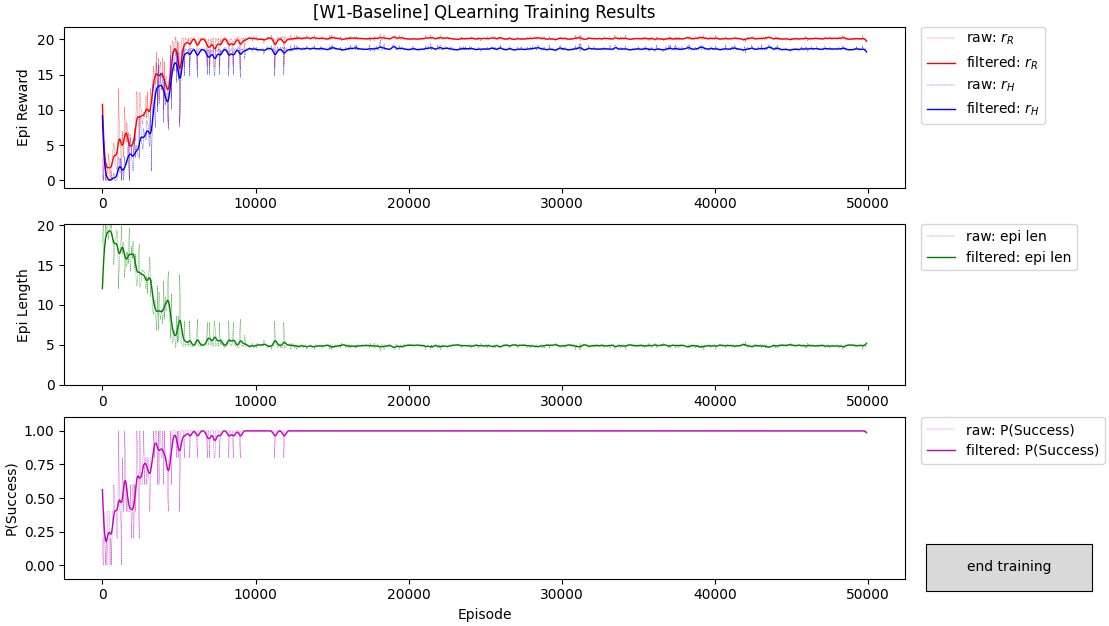
\includegraphics[width=\textwidth]{Prog4_Jan7/materials/Fig_W1_JointQ_Baseline.png}
        %      \caption{Optimal} \label{fig:W1baseline}
        %  \end{subfigure}
        %  \hfill
         \begin{subfigure}[b]{\Wfig\textwidth} \centering
             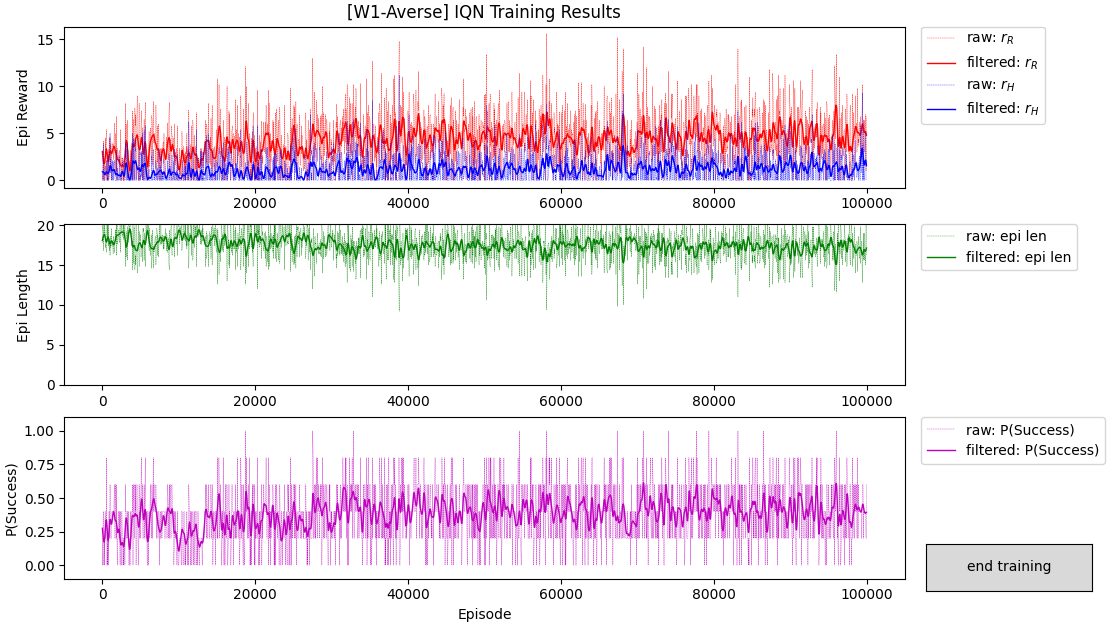
\includegraphics[width=\textwidth]{../results/IDQN_W1/Fig_W1_JointQ_Averse}
             \caption{Risk-Averse} \label{fig:W1averse}
         \end{subfigure}
         \hfill
         \begin{subfigure}[b]{\Wfig\textwidth} \centering
             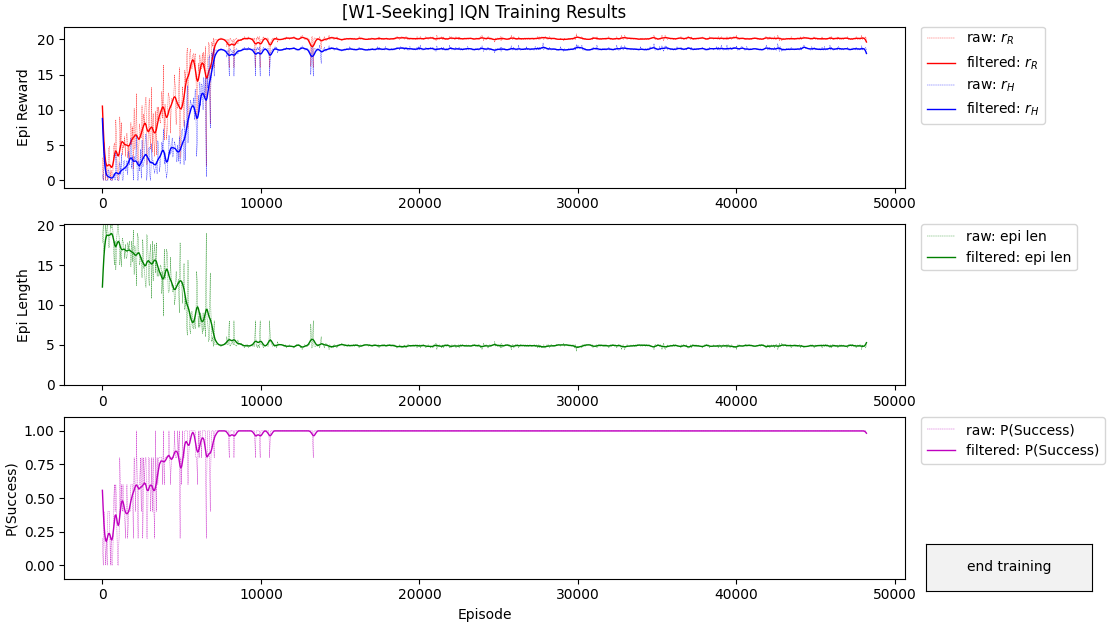
\includegraphics[width=\textwidth]{../results/IDQN_W1/Fig_W1_JointQ_Seeking}
             \caption{Risk-Seeking} \label{fig:W1seeking}
         \end{subfigure}
    \caption{World 1 Training Results}
    \label{fig:W1}
    \end{figure}
\end{frame}

\begin{frame}{Training Results (World 2)}
     \begin{figure}
     \centering
        %  \begin{subfigure}[b]{\Wfig\textwidth}  \centering
        %      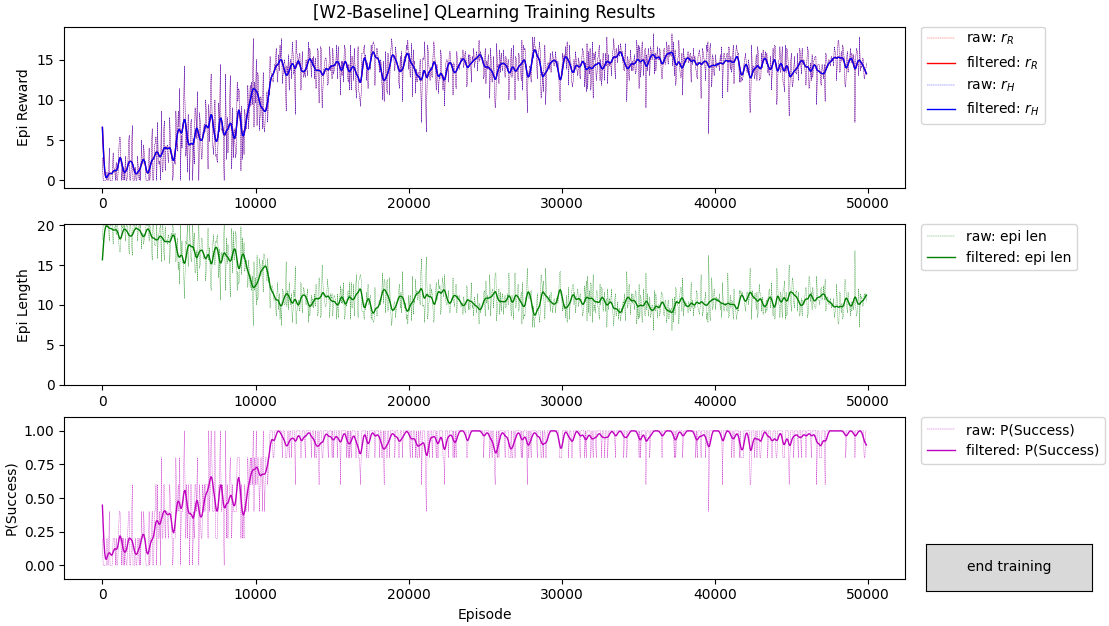
\includegraphics[width=\textwidth]{Prog4_Jan7/materials/Fig_W2_JointQ_Baseline.png}
        %      \caption{Optimal} \label{fig:W2baseline}
        %  \end{subfigure}
        %  \hfill
         \begin{subfigure}[b]{\Wfig\textwidth} \centering
             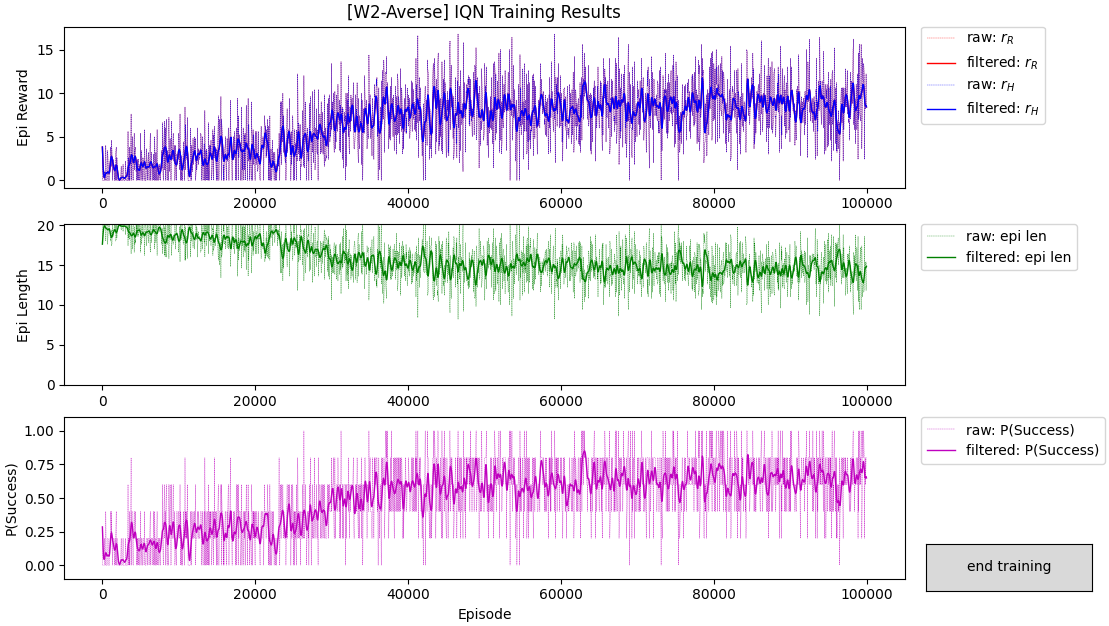
\includegraphics[width=\textwidth]{../results/IDQN_W2/Fig_W2_JointQ_Averse}
             \caption{Risk-Averse} \label{fig:W2averse}
         \end{subfigure}
         \hfill
         \begin{subfigure}[b]{\Wfig\textwidth} \centering
             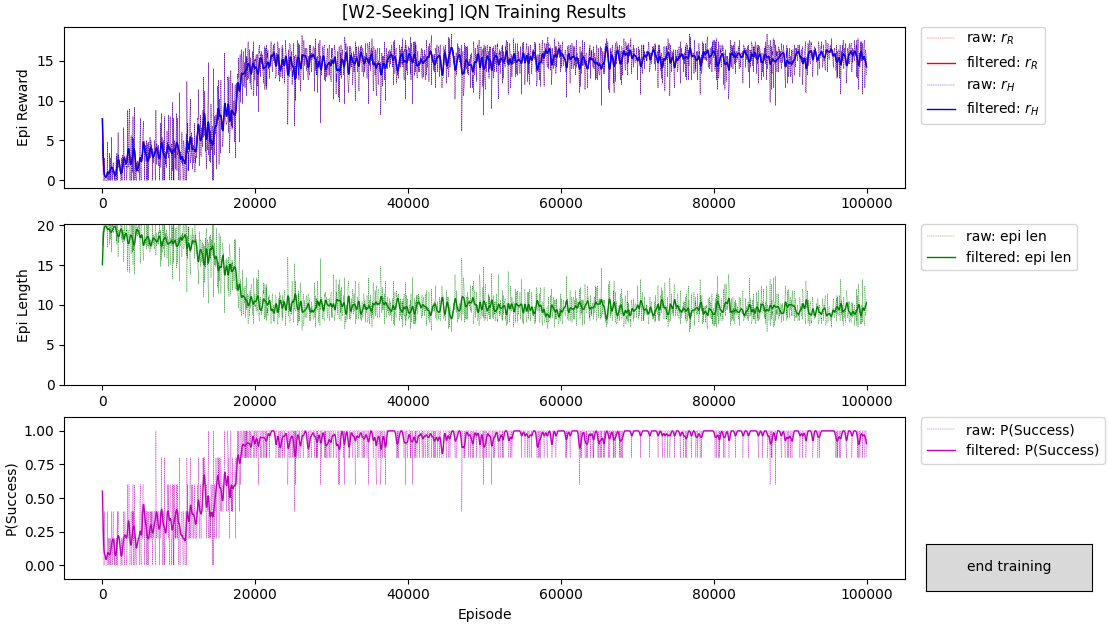
\includegraphics[width=\textwidth]{../results/IDQN_W2/Fig_W2_JointQ_Seeking}
             \caption{Risk-Seeking} \label{fig:W2seeking}
         \end{subfigure}
    \caption{World 2 Training Results}
    \label{fig:W2}
    \end{figure}
\end{frame}


\begin{frame}{Training Results (World 3)}
     \begin{figure}
     \centering
        %  \begin{subfigure}[b]{\Wfig\textwidth}  \centering
        %      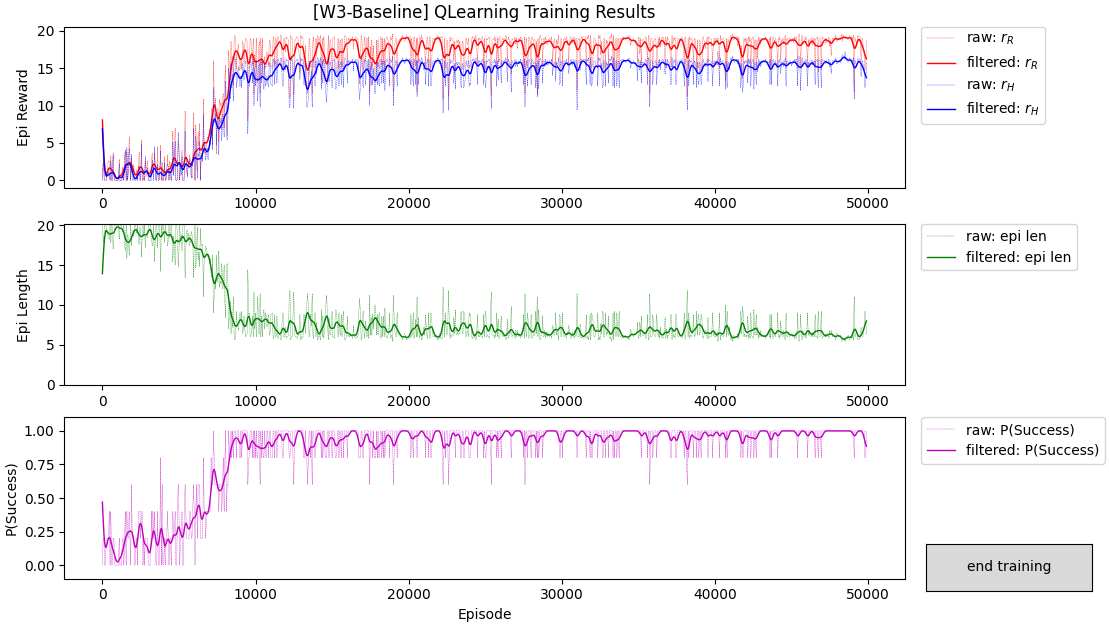
\includegraphics[width=\textwidth]{Prog4_Jan7/materials/Fig_W3_JointQ_Baseline.png}
        %      \caption{Optimal} \label{fig:W3baseline}
        %  \end{subfigure}
        %  \hfill
         \begin{subfigure}[b]{\Wfig\textwidth} \centering
             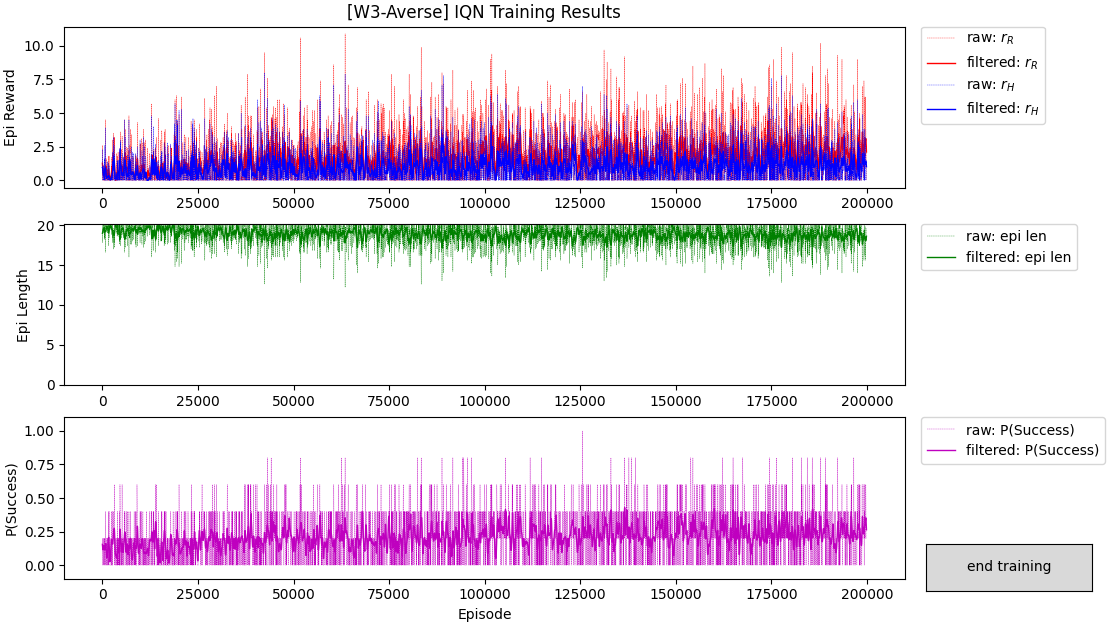
\includegraphics[width=\textwidth]{../results/IDQN_W3/Fig_W3_JointQ_Averse}
             \caption{Risk-Averse} \label{fig:W3averse}
         \end{subfigure}
         \hfill
         \begin{subfigure}[b]{\Wfig\textwidth} \centering
             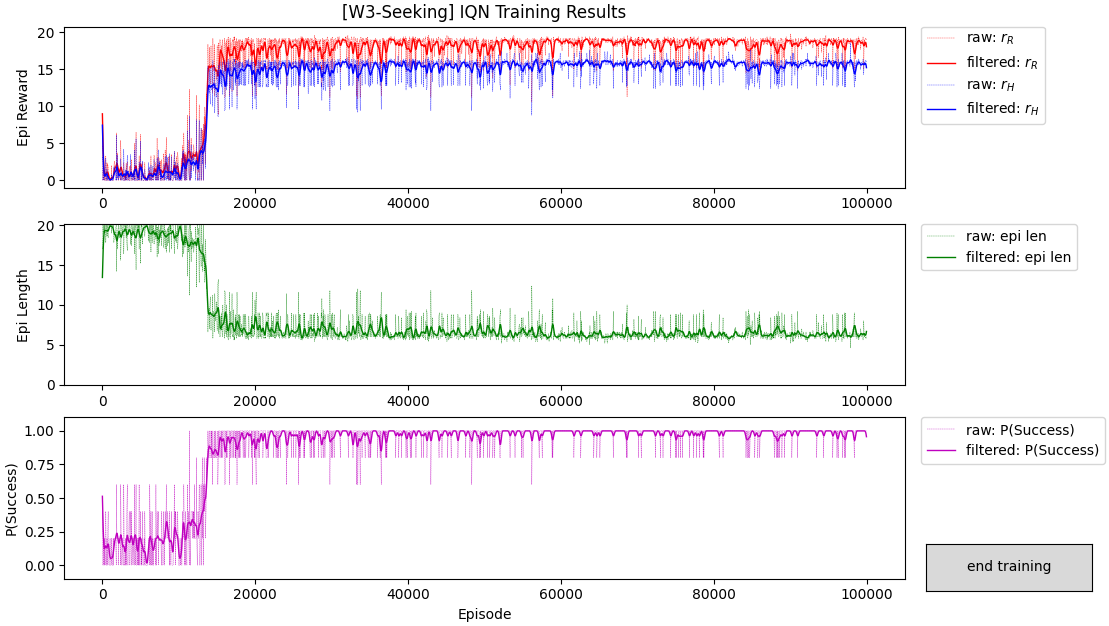
\includegraphics[width=\textwidth]{../results/IDQN_W3/Fig_W3_JointQ_Seeking}
             \caption{Risk-Seeking} \label{fig:W3seeking}
         \end{subfigure}
    \caption{World 3 Training Results}
    \label{fig:W3}
    \end{figure}
\end{frame}


\begin{frame}{Training Results (World 4)}
     \begin{figure}
     \centering
        %  \begin{subfigure}[b]{\Wfig\textwidth}  \centering
        %      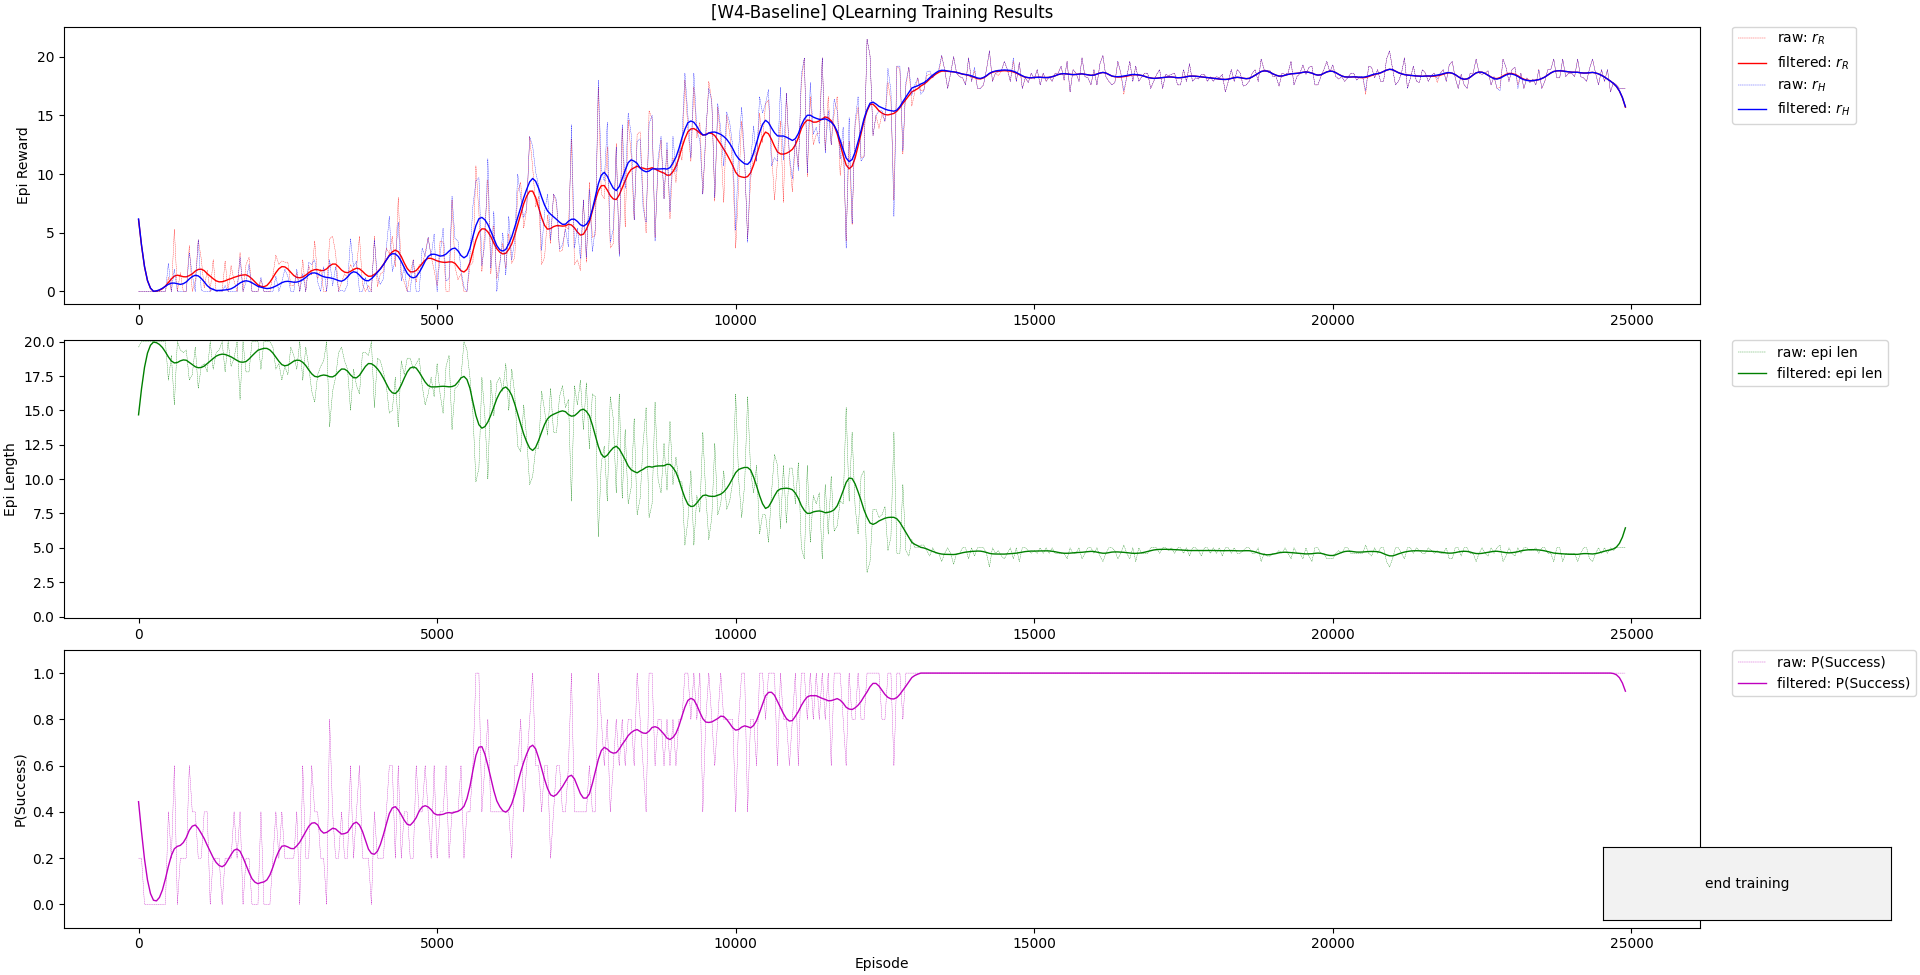
\includegraphics[width=\textwidth]{Prog4_Jan7/materials/Fig_W4_JointQ_Baseline.png}
        %      \caption{Optimal} \label{fig:W4baseline}
        %  \end{subfigure}
        %  \hfill
         \begin{subfigure}[b]{\Wfig\textwidth} \centering
             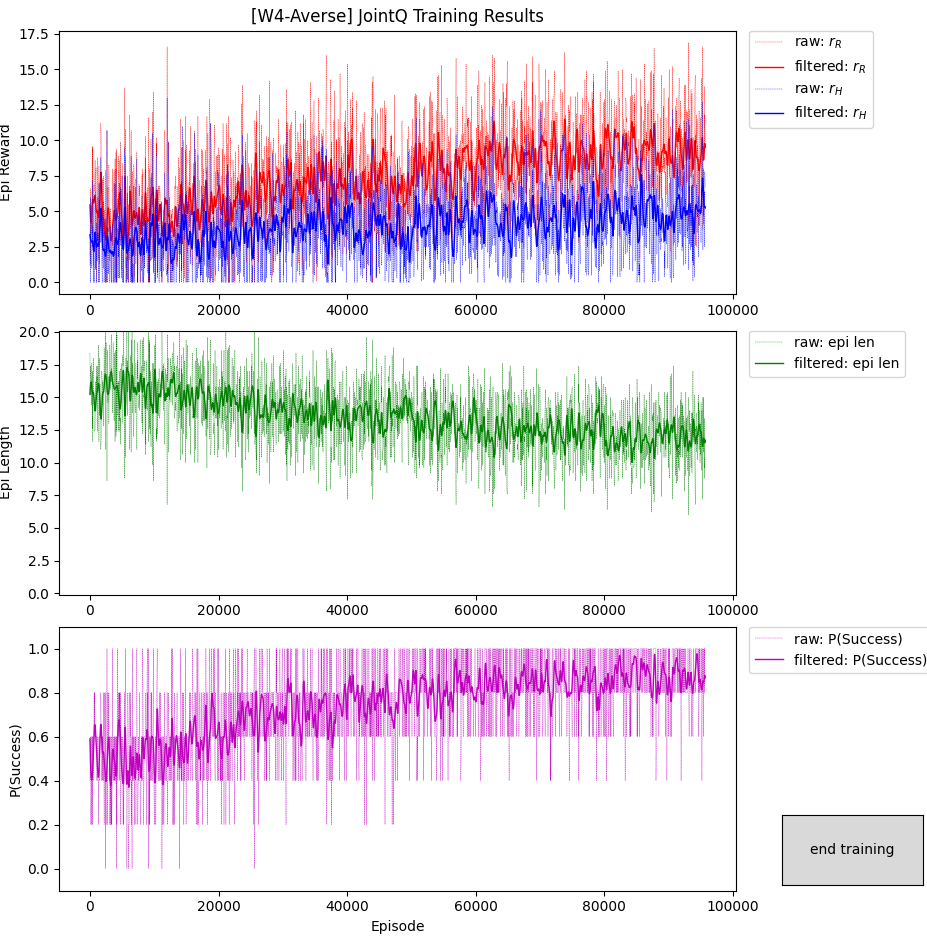
\includegraphics[width=\textwidth]{../results/IDQN_W4/Fig_W4_JointQ_Averse}
             \caption{Risk-Averse} \label{fig:W4averse}
         \end{subfigure}
         \hfill
         \begin{subfigure}[b]{\Wfig\textwidth} \centering
             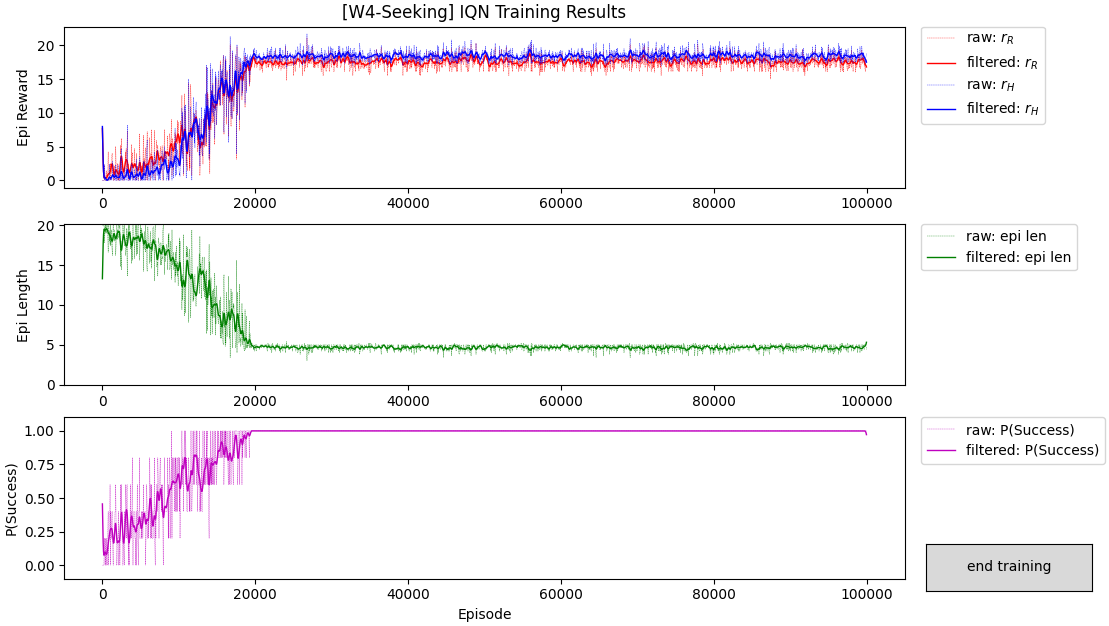
\includegraphics[width=\textwidth]{../results/IDQN_W4/Fig_W4_JointQ_Seeking}
             \caption{Risk-Seeking} \label{fig:W4seeking}
         \end{subfigure}
    \caption{World 4 Training Results}
    \label{fig:W4}
    \end{figure}
\end{frame}


\begin{frame}{Training Results (World 5)}
     \begin{figure}
     \centering
        %  \begin{subfigure}[b]{\Wfig\textwidth}  \centering
        %      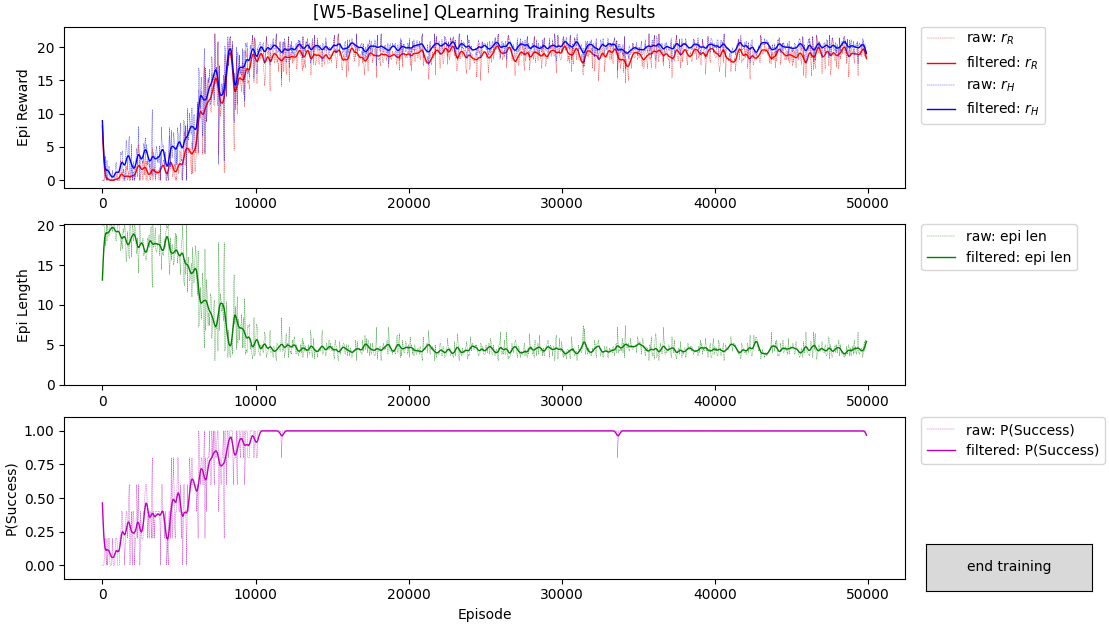
\includegraphics[width=\textwidth]{Prog4_Jan7/materials/Fig_W5_JointQ_Baseline.png}
        %      \caption{Optimal} \label{fig:W5baseline}
        %  \end{subfigure}
        %  \hfill
         \begin{subfigure}[b]{\Wfig\textwidth} \centering
             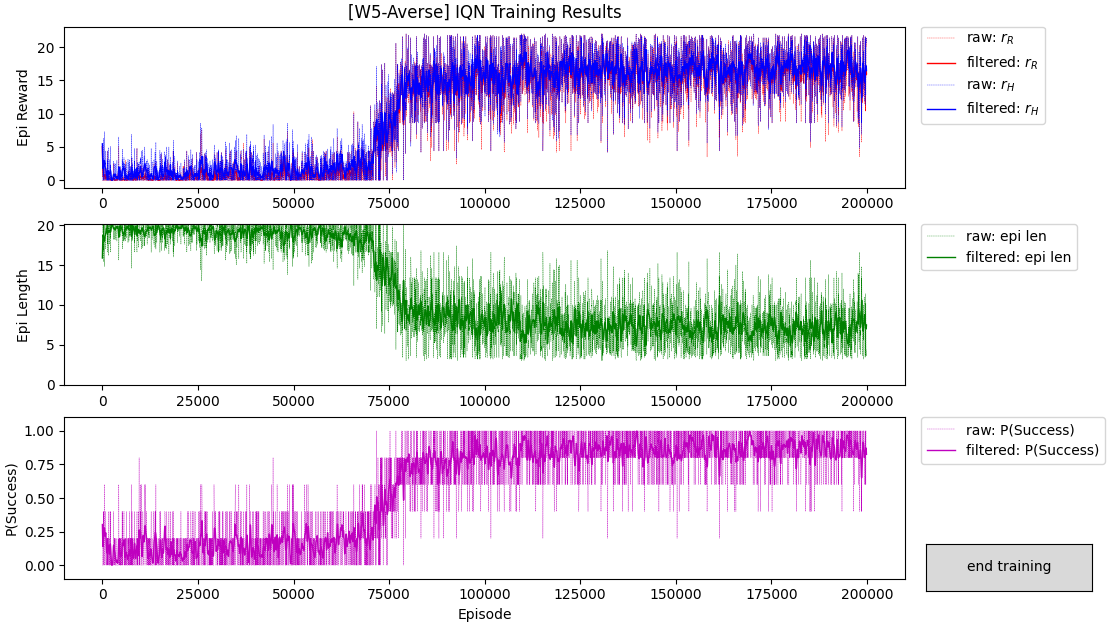
\includegraphics[width=\textwidth]{../results/IDQN_W5/Fig_W5_JointQ_Averse}
             \caption{Risk-Averse} \label{fig:W5averse}
         \end{subfigure}
         \hfill
         \begin{subfigure}[b]{\Wfig\textwidth} \centering
             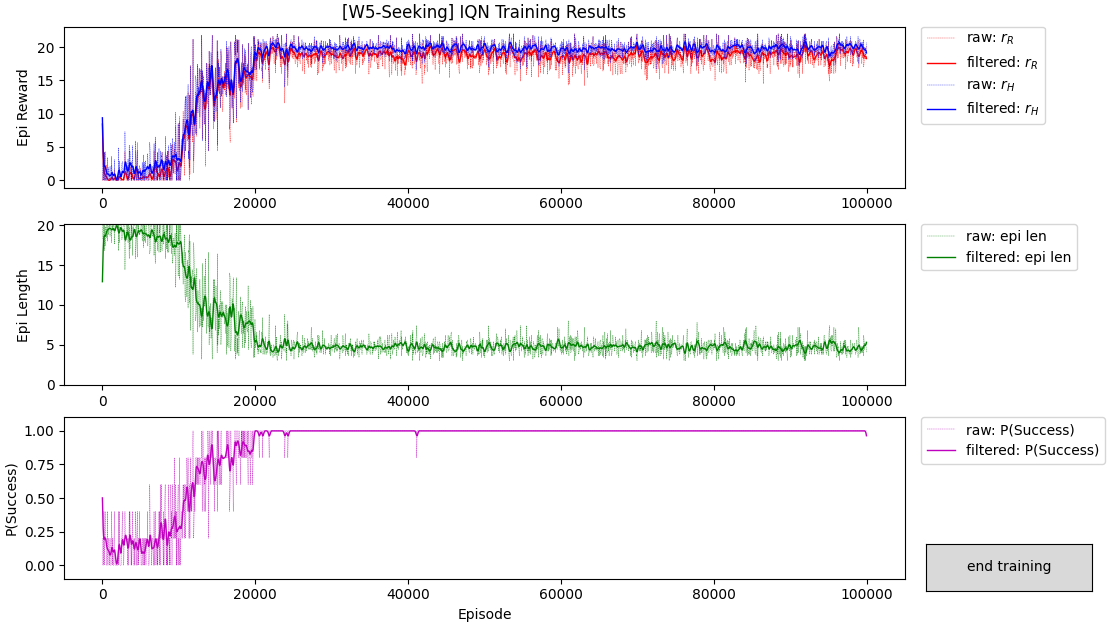
\includegraphics[width=\textwidth]{../results/IDQN_W5/Fig_W5_JointQ_Seeking}
             \caption{Risk-Seeking} \label{fig:W5seeking}
         \end{subfigure}
    \caption{World 5 Training Results}
    \label{fig:W5}
    \end{figure}
\end{frame}

\begin{frame}{Training Results (World 6)}
     \begin{figure}
     \centering
        %  \begin{subfigure}[b]{\Wfig\textwidth}  \centering
        %      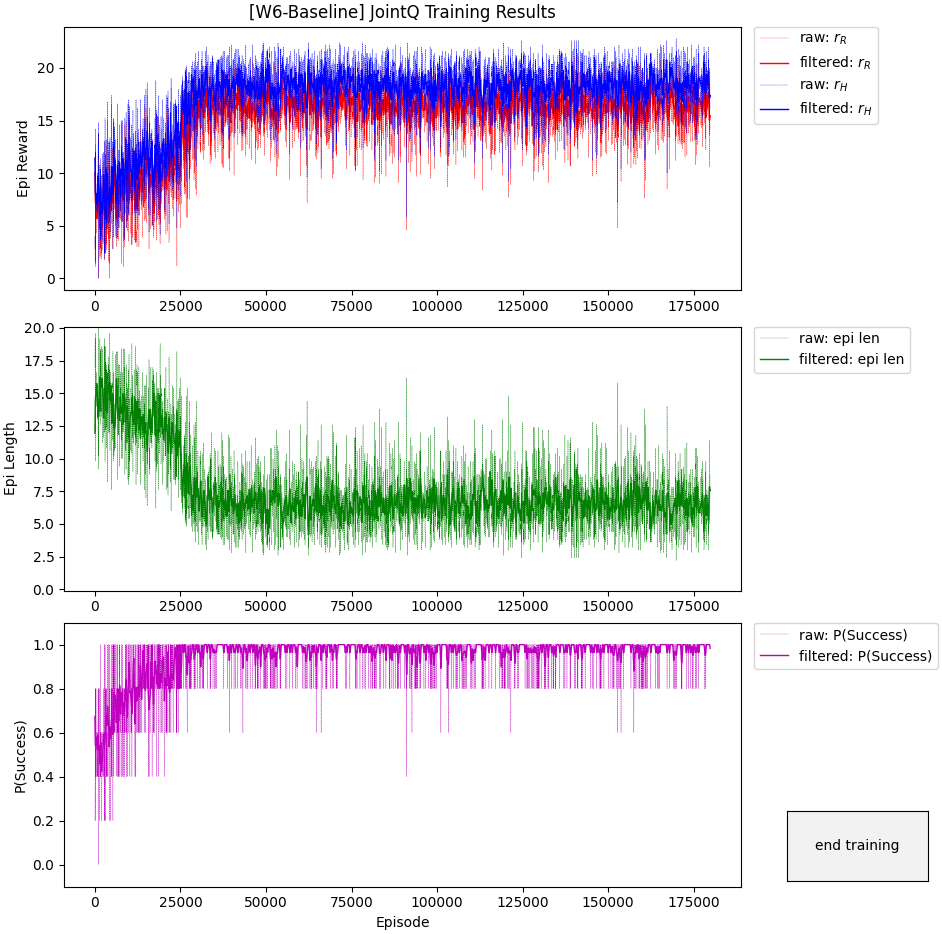
\includegraphics[width=\textwidth]{Prog4_Jan7/materials/Fig_W6_JointQ_Baseline.png}
        %      \caption{Optimal} \label{fig:W6baseline}
        %  \end{subfigure}
        %  \hfill
         \begin{subfigure}[b]{\Wfig\textwidth} \centering
             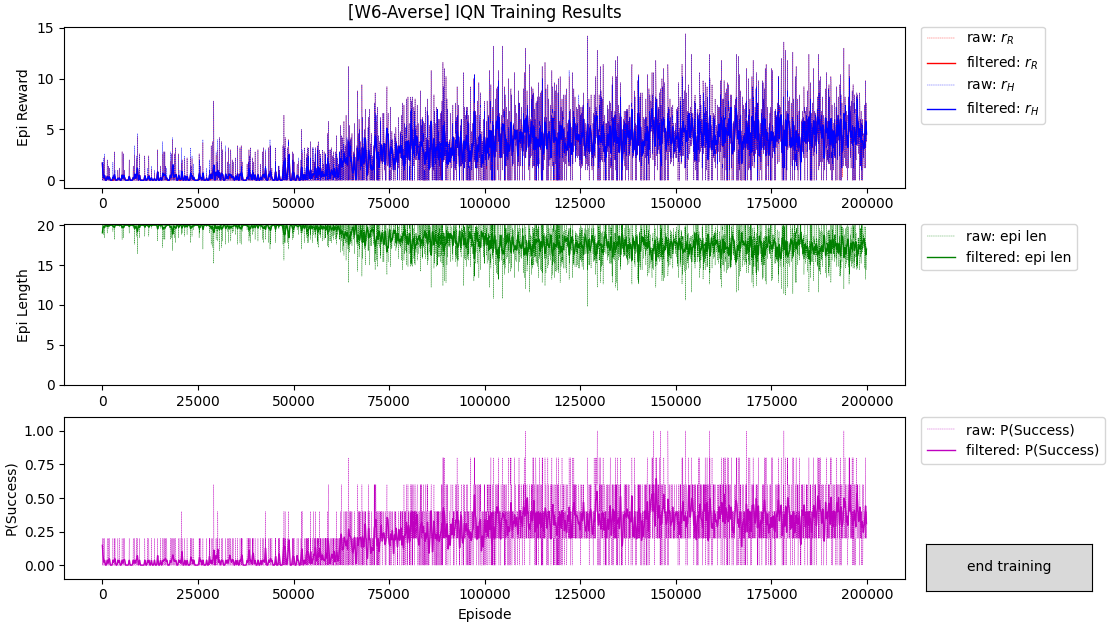
\includegraphics[width=\textwidth]{../results/IDQN_W6/Fig_W6_JointQ_Averse}
             \caption{Risk-Averse} \label{fig:W6averse}
         \end{subfigure}
         \hfill
         \begin{subfigure}[b]{\Wfig\textwidth} \centering
             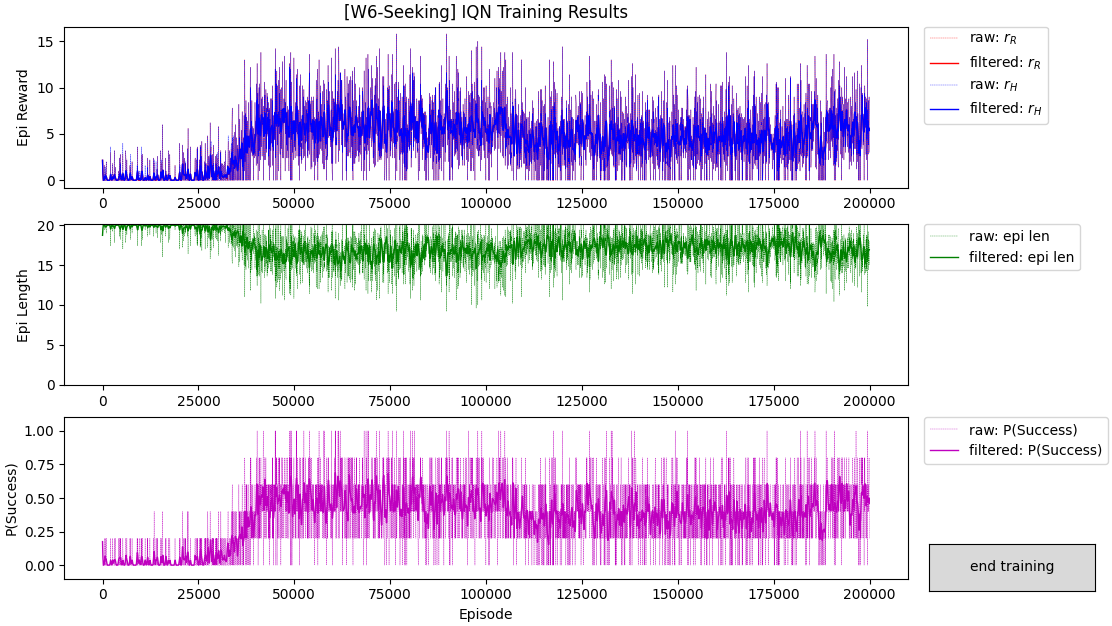
\includegraphics[width=\textwidth]{../results/IDQN_W6//Fig_W6_JointQ_Seeking}
             \caption{Risk-Seeking} \label{fig:W6seeking}
         \end{subfigure}
    \caption{World 6 Training Results}
    \label{fig:W6}
    \end{figure}
\end{frame}


% \begin{frame}{Training Results (World 7)}
%      \begin{figure}
%      \centering
        %  \begin{subfigure}[b]{\Wfig\textwidth}  \centering
        %      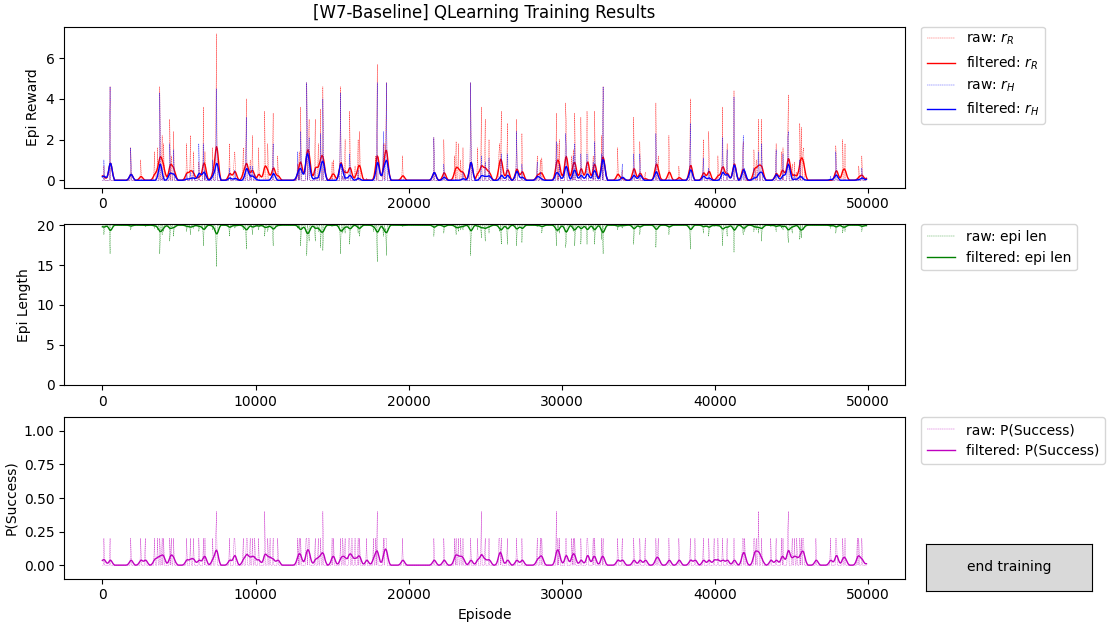
\includegraphics[width=\textwidth]{Prog4_Jan7/materials/Fig_W7_JointQ_Baseline.png}
        %      \caption{Optimal} \label{fig:W7baseline}
        %  \end{subfigure}
        %  \hfill
%          \begin{subfigure}[b]{\Wfig\textwidth} \centering
%              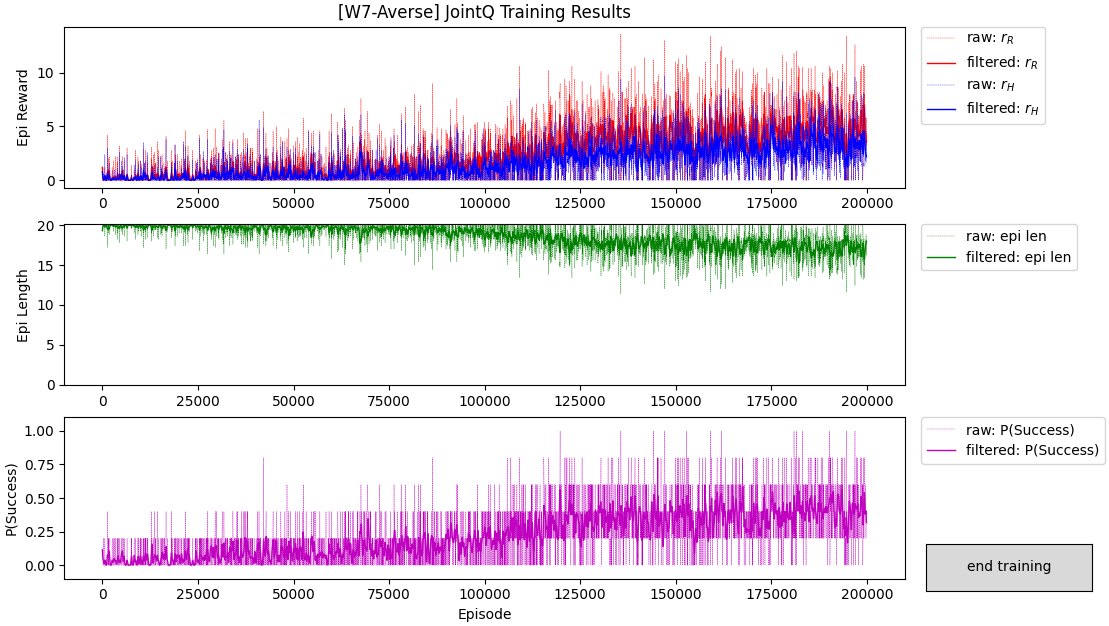
\includegraphics[width=\textwidth]{Prog4_Jan7/materials/Fig_W7_JointQ_Averse.png}
%              \caption{Risk-Averse} \label{fig:W7averse}
%          \end{subfigure}
%          \hfill
%          \begin{subfigure}[b]{\Wfig\textwidth} \centering
%              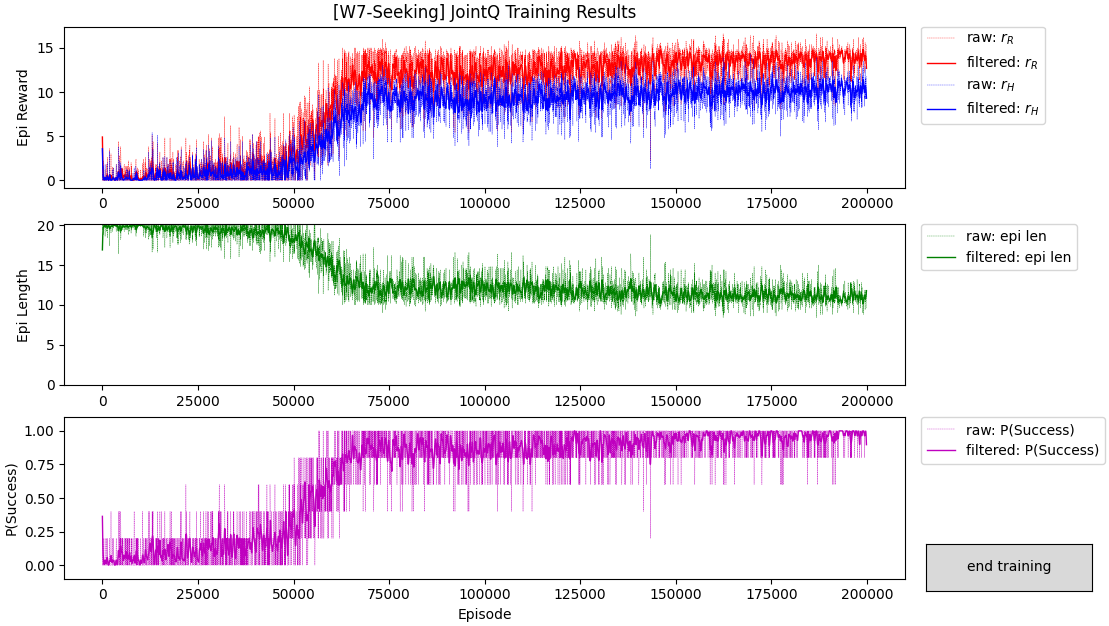
\includegraphics[width=\textwidth]{Prog4_Jan7/materials/Fig_W7_JointQ_Seeking.png}
%              \caption{Risk-Seeking} \label{fig:W7seeking}
%          \end{subfigure}
%     \caption{World 7 Training Results}
%     \label{fig:W7}
%     \end{figure}
% \end{frame}


\subsection{Discussion}\label{subsec:discussion}\begin{frame}{Discussion}
\begin{itemize}
    \item Policies are generally noisy due not non-stationary and rationality constant = 1
    \item Equilibrium would be less stochastic with higher rationalities
    \item Noise in final result pseudo-required to avoid the previously mentioned all or nothing problem (e.i. there exists dis-coordination and vulnerability to partner uncertainty)
    \item Baseline (Optimal) policies are often similar to Risk-Seeking policies since the game is designed for the agents to succeed
    \begin{itemize}
        \item Rushing through penalties is often a good strategy
        \item Susceptible to partner and target stochasticity
    \end{itemize}
    \item May make minor attempts to improve policies in future but this is good for now
\end{itemize}
\end{frame}
%#########################################################
%#########################################################
%#########################################################
\section{Simulation}\label{sec:simulation} \displayTOC
\subsection{Formulation}
\begin{frame}{Setup}
    Goal: \begin{itemize}
        \item Evaluate how assumptions of H's risk-sensitivity effect team performance
        \item Provide validation that there are differing or conflicting optimal policies based on risk-sensitivity
    \end{itemize}
    Experimental Conditions: \begin{itemize}
        \item We manipulate
        \begin{itemize}
            \item what R assumes H's policy to be ($\hat{\pi}_{H}$)
            \item what H's policy actually is ($\pi_{H}$)
        \end{itemize}
        \item The experimental condition is then written as $\mathcal{C} = \{\hat{\pi}_{H},\pi_{H}\}$
        \item Substituting in our bias policies that we trained we get four conditions:
        \begin{itemize}
            \item Assume-Averse + Is-Averse:  $\{\hat{\pi}_{A},\pi_{A}\}$ (Correct Assumption)
            \item Assume-Seeking + Is-Averse:  $\{\hat{\pi}_{S},\pi_{A}\}$ (Incorrect Assumption)
            \item Assume-Averse + Is-Seeking:  $\{\hat{\pi}_{A},\pi_{S}\}$ (Incorrect Assumption)
            \item Assume-Seeking + Is-Seeking:  $\{\hat{\pi}_{S},\pi_{S}\}$ (Correct Assumption)
            \item \textit{can include optimal vs X conditions but small effect is present}
        \end{itemize}

    \end{itemize}
\end{frame}

\begin{frame}{Analysis}
    Approach: \begin{itemize}
        \item We \textbf{only compare between R's assumption} and within H's actually policy
        \item H's actually policy directly effects game performance and invalidates some evaluation metrics
        \item R's policy will be $\pi_R=\pi_0$ conditioned on $\hat{\pi}_{H}$ using \ac{QRE}
        \item H will assume R uses H's true policy $\hat{\pi}_{R}=\pi_{H}$
        \item Run simulated game 1000x for each of the 4 conditions composed
    \end{itemize}
    Metrics: \begin{itemize}
        \item Each agent's reward and the team (mean) reward between assumptions
        \item Episode length and probability of catching the target between assumptions
        \item Number of penalty states each agent during an average game between assumptions
        \item Mean probability of partner's action in ego's mental model $p(a_{-k} | \hat{\pi}_{-k})$
    \end{itemize}
\end{frame}


\subsection{Hypothesis}
\begin{frame}{Hypothesis}
    \begin{itemize}
        \item When R assumes wrong ($\hat{\pi}_H \neq \pi_H$) for both $\pi_H \in (\pi_A,\pi_S)$: % due to discoordination
        \begin{itemize}
            \item[\textbf{H1.1}:] Each agent's and team reward will decrease
            \item[\textbf{H1.2}:] Episode length will increase
            \item[\textbf{H1.3}:] Probability of catching target will decrease
            \item[\textbf{H1.3}:] Number of penalty states entered will increase
            \item[\textbf{H1.4}:] Both agents will not be able to predict each other's actions well (small  $p(a_{-k} | \hat{\pi}_{-k})$)
        \end{itemize}
    \item[]
    \item When H is averse ($\pi_H = \pi_A$) instead of seeking: % due to discoordination
        \begin{itemize}
            \item[\textbf{H2.1}:] Magnitude of performance losses will be less significant
            \item[\textbf{H2.2}:] Performance will be worse than if $\pi_H = \pi_S$
            % \item[\textbf{H2.3}:]
            % \item[\textbf{H2.3}:]
        \end{itemize}
    \item[]
    \item Misc. Hypothesises\begin{itemize}
        \item[\textbf{H3}:] Only minor changes in terminal state location will occur when agents succeed (e.i. objective remains the same but joint-trajectory changes).
    \end{itemize}
    \end{itemize}
\end{frame}


\subsection{Analysis}
\begin{frame}{Analysis}
    Metrics: \begin{itemize}
        \item
    \end{itemize}
    \begin{itemize}
        \item * on top of bars and in key indicate correct assumption made
    \end{itemize}
\end{frame}


\subsection{Results}
\begin{frame}{Results}
     \begin{figure} \centering
        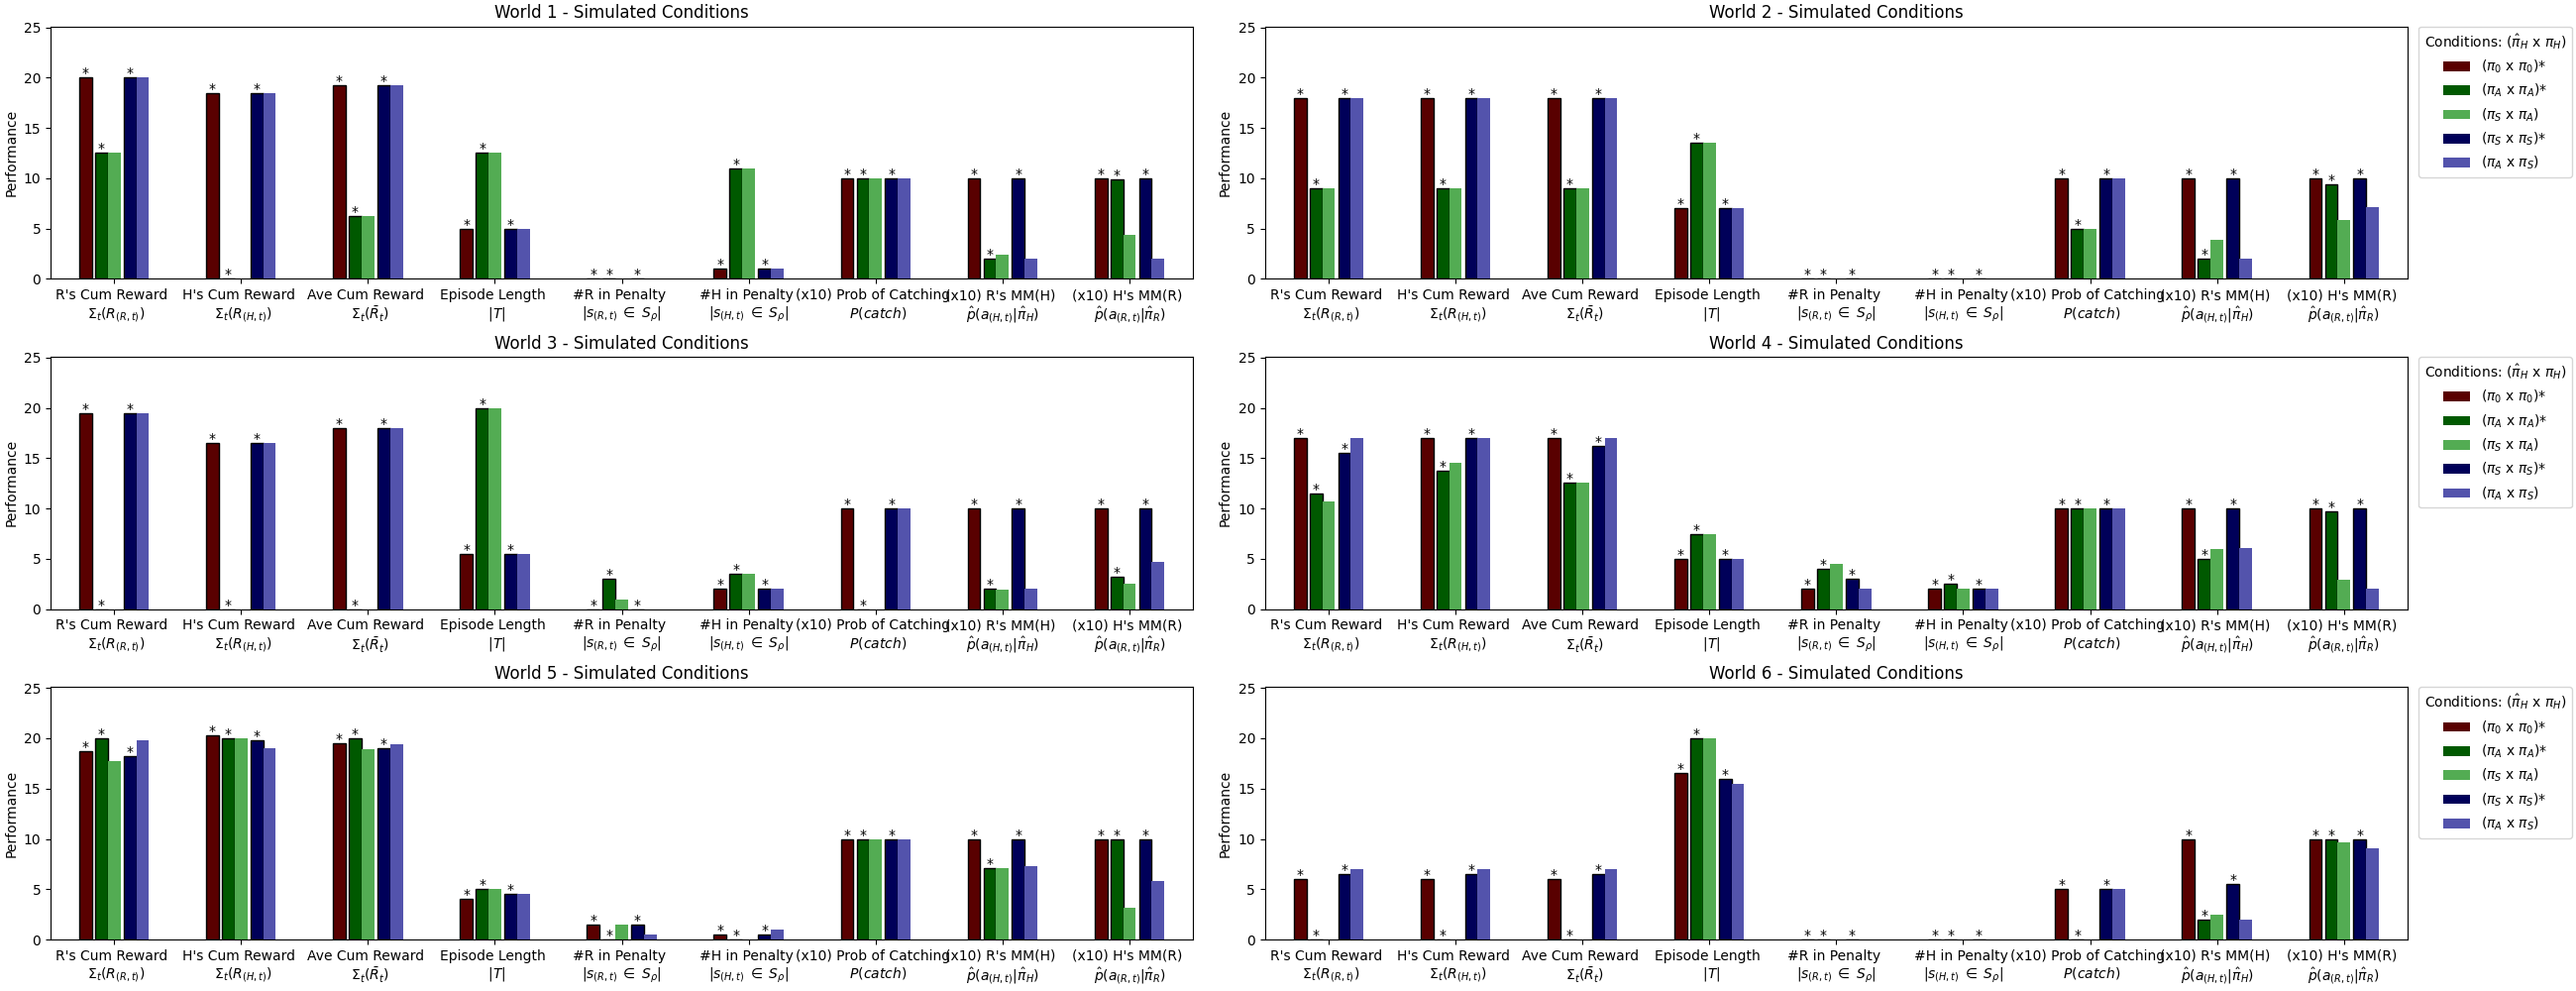
\includegraphics[width=0.99\textwidth]{../results/policy_comparisons/Fig_AssumptionComparison}
        \caption{Evaluation of simulated conditions per world}
        \label{fig:PolicyCompWorld}
    \end{figure}
\end{frame}
\begin{frame}{Results}
     \begin{figure} \centering
        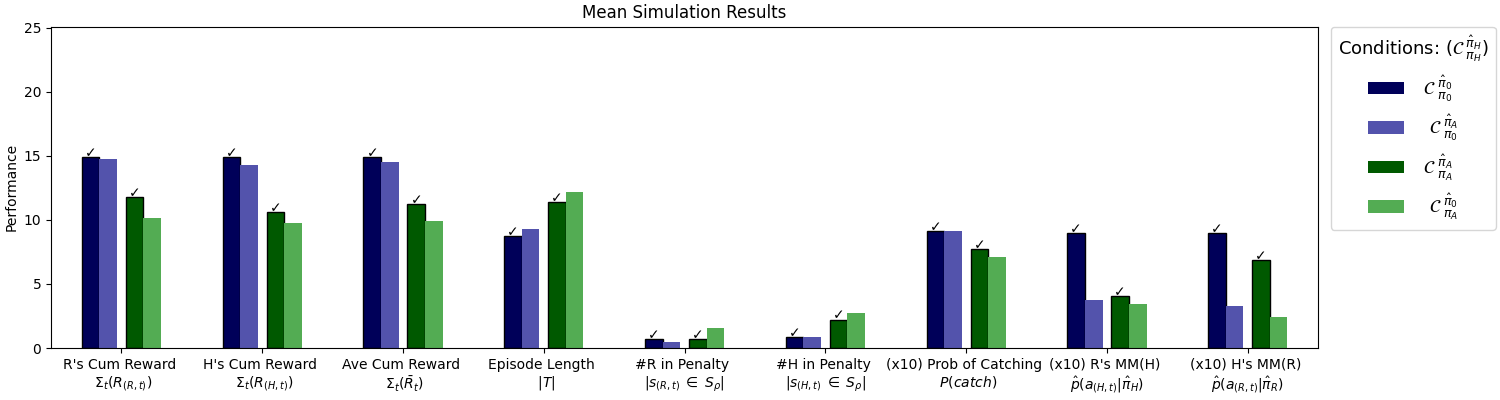
\includegraphics[width=0.99\textwidth]{../results/policy_comparisons/Fig_AssumptionComparison_Summary}
        \caption{Evaluation of simulated conditions summary}
        \label{fig:PolicyCompSummary}
    \end{figure}
\end{frame}

\subsection{Discussion}
\begin{frame}{Discussion}
\begin{itemize}
    \item \add{ADD DISCUSSION}
\end{itemize}
\end{frame}

%#########################################################
%#########################################################
%#########################################################

\section{Upcoming Work} \displayTOC
\begin{frame}{2-Week Sprint Goals}
    Goal: \begin{itemize}
        \item Description
    \end{itemize}
\end{frame}


\begin{frame}{Long-Term Goals}
    Goal: \begin{itemize}
        \item Description
    \end{itemize}
\end{frame}

% \section{Conclusion}
% \subsection{Timeline}
\end{document}